\documentclass[preprint,12pt]{elsarticle}


\usepackage[spanish]{babel}
\usepackage{amssymb}
\usepackage{graphicx}
\usepackage{lineno}
\usepackage[utf8]{inputenc}
\usepackage{url}
\usepackage{cite} 




\journal{Data Story Telling}

\begin{document}
	\begin{frontmatter}
		
		
		\title{\huge Data Story Telling}
		
		
		\author{Escalante Maron, Nelia (2014049551)  
			\\Condori Gutierrez, Flor (2015053227)
			\\Coaquira Calizaya, Yerson (2015053225)
			\\Cespedes Medina, Christian (2010036256)   
			\\Arteaga Ramos, Javier Octavio (2007028981)  }
		
		\address{Tacna, Peru}
		
				
		\begin{abstract}
			
			%% Text of abstract
			El mundo de la visualización de datos es fascinante, pero el éxito de una buena visualización no solo radica en el análisis y creación de gráficas con datos sino más bien en la organización de la información y la narrativa de los mismos. 
			El data storytelling, tal como lo señala GlobalWebIndex, se trata de generar conexiones usando datos como la fuente que guíe a la marca. Ya sea que se emplee para dar forma a una identidad de marca única o para generar una campaña de marketing de impacto, el data storytelling aporta a las marcas la oportunidad de capturar la atención de una forma que se centra enteramente en la audiencia objetivo. Las historias que están formadas de esta forma son las que logran darles vida a las marcas.\\
			
			\textit{The world of data visualization is fascinating, but the success of a good visualization not only lies in the analysis and creation of graphs with data but rather in the organization of the information and the narrative thereof.
			Data storytelling, as GlobalWebIndex points out, is about generating connections using data as the source that guides the brand. Whether used to shape a unique brand identity or to generate an impact marketing campaign, data storytelling gives brands the opportunity to capture attention in a way that focuses entirely on the target audience. The stories that are formed in this way are those that manage to give life to the brands.}
						
		\end{abstract}
		
	\end{frontmatter}
	%%
	%% Start line numbering here if you want
	%%
	%\linenumbers
	
	%% main text
	\newpage
	\section{INTRODUCCION}
	\label{S:1}
	El Data Storytelling es una herramienta que emplea la combinación de datos estadísticos y comunicación. Ayuda a las empresas a cumplir metas de comunicación y marketing contando mensajes de manera efectiva y cargados de información relevante para el público objetivo, también apoyados en instrumentos visuales y narrativos.\\
	\\
	Para poder llevar a cabo la implementación del Data Storytelling, es necesario contar con algunas herramientas de tecnologías de la información, tales como: base de datos que nos permitirá comprender el comportamiento y contextos de los grupos a los que queremos dirigirnos, buscaremos datos que nos permitan generar un insight en común, esta base de datos se puede enriquecer, a través de encuestas o formularios brindados por los grupos de interés, es indispensable contar con computadoras y tablets que apoyen la elaboración del contenido a presentar.\\
	\\
	Se pueden emplear las diferentes redes sociales para difundir las historias con los respectivos mensajes que queremos hacer llegar a nuestros grupos objetivos, es por esto que también es necesario poder conocer los máximos beneficios que éstas pueden ofrecer, ya que de nada serviría enviar los mensajes a personas que no formen parte del grupo al que queremos llegar.
	
	\section{OBJETIVOS}
		\begin{enumerate}[a)]
			\item Las historias son herramientas efectivas para transmitir la experiencia humana: esto ha sido así desde el inicio de los tiempos, pero ahora utilizamos datos y análisis para crear versiones mejoradas de esas historias. Gracias a ellas simplificamos y damos sentido a un mundo complejo.
			\\
			\item Para inspirar el cambio, necesitamos que entiendan nuestra historia: no importa cuántas horas hay detrás de nuestro análisis, no lograremos nada si no nos logramos explicar ya sea con una narrativa o con gráficos pero, necesitamos una historia.
			\\
			\item Las personas quieren evidencia del análisis que hay detrás: aunque nuestra audiencia no entienda el detalle de la analítica, sí quieren la evidencia de que hay datos detrás, ya que estas historias son más convincentes que solo una experiencia personal.
			\\
			\item Contar en una breve historia el resultado de horas de trabajo: se necesitan presentaciones cortas, con ideas concretas adaptadas a los stakeholders que recibirán la información para hacer llegar tu mensaje de una manera simple. 
		\end{enumerate}
	
	\section{MARCO TEÓRICO}
	\textbf{ STORY TELLING}\\
	
	Philippe Nieuwbourg: “El Storytelling es el arte y la manera de contar una historia dándoles un toque humano y el Data Storytelling es el arte y la manera de contar una historia apoyándose en los datos, cifras, o hechos, ya que si tomamos una gráfica o una simple curva ésta no cuenta ninguna historia. Entonces, el Data Storytelling ayuda a crear una historia que permitirá explicar las cifras y los datos”. \\
	\\
	Por ponerlo de una forma más simple, la firma Analítica Web señala que el llamado data storytelling no es más que un enfoque estructurado sobre cómo se comunican insights a partir de datos, este enfoque se vale de datos, visualización y narrativa, y la combinación de estos elementos deriva en distintos resultados, por ejemplo, la suma de la narrativa y los datos permite “explicar”, la suma de la visualización y los datos, permite “ilustrar”, y la suma de la narrativa con la visualización aporta como resultado el “entretenimiento”. La suma de los tres elementos arroja como resultado un el concepto de “cambio”. [\citen{bib01}]\\

\textbf{ELEMENTOS CLAVE DEL DATA STORYTELLING}\\
	
	El llamado Data Storytelling no es más que un enfoque estructurado sobre cómo comunicamos insights a partir de los datos, e involucra una combinación de tres elementos: 
	\begin{itemize}
		\item Ciencia de los Datos o datos
			
		Tal como lo destacamos hace poco la data science o ciencia de datos consiste en la práctica de revelar insights ocultos en los datos existentes aun una forma que habilite a las empresas a tomar mejores decisiones se trata de un concepto que puede ayudar a mejorar el rendimiento y crecimiento de un negocio.
		
		
		\item Visualizaciones
		
		Transformar data en gráficos, tablas o formatos similares significa que se puede visualizar la data como una antes. Las visualizaciones ahora son posibles y mejores gracias a las soluciones de tecnologías emergentes que nos ayudan a comprender cantidades importantes de información recolectada.  Las visualizaciones de datos por sí solas tienen limitaciones, por ello, el tercer campo de exprese es la narrativa.
		
		\item Narrativa
		
		Dentro del data storytelling, la narrativa se puede considerar el elemento más importante. La narrativa utiliza el lenguaje en un formato que se adecua a ciertas necesidades en particular aumentando la comprensión de nueva información, es el vehículo clave para transmitir insights.\\
		\\
		Resultado de las uniones de los elementos:
		
		\begin{center}
			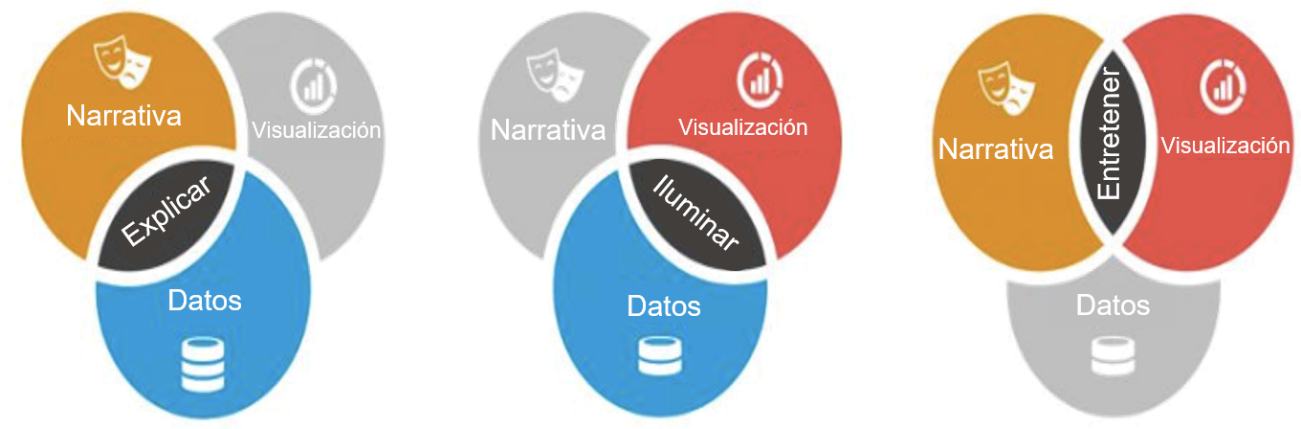
\includegraphics[width=13cm]{./Imagenes/img1} 
		\end{center}
		
			\begin{itemize}
				\item Narrativa + Datos = Explicar. Podremos explicar qué ha pasado y por qué un insight puede ser importante. Necesitaremos contexto para entender las conclusiones por completo.
				\item Visualización + Datos = Iluminar. Cuando añadimos una visualización a nuestros datos, podemos iluminar a nuestra audiencia con insights que no habrían visto de otra manera.
				\item Narrativa + Visualización = Entretener. La combinación perfecta para lograr ese interés e incluso para entretener a nuestra audiencia.
			\end{itemize}

	\end{itemize}
	Cuando se reúne la Visualización + Narración + Datos = Cambio, se logra contar una historia con datos, se logra influenciar y llevar a ese cambio que se está buscando [\citen{bib02}].
	
	\begin{center}
		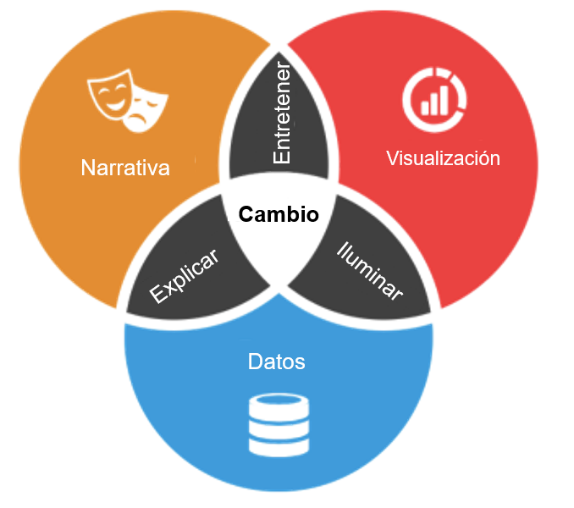
\includegraphics[width=7cm]{./Imagenes/img2} 
	\end{center}

	\section{IMPORTANCIA}
	
	Contar una gran historia basada en datos puede ser útil tanto para las partes interesadas como para sus clientes y puede impulsar una mejor toma de decisiones dentro de una organización y también impulsar conversiones con sus clientes. Al utilizar la visualización de datos para hacer observaciones clave sobre sus clientes y sus necesidades, puede ayudar a generar clientes potenciales y retener clientes.\\
	\\
	Algunas de las razones por las que es importante emplear esta herramienta dentro de una organización, o de manera personal, son las siguientes:
	
	\begin{itemize}
		\item En primer lugar, la importancia radica en la riqueza de la información con la que se cuenta dentro de una base de datos y el aporte que ésta brinda al momento de contar una historia.
		\item También permite simplificar toda la información que las organizaciones quieren transmitir a sus diferentes grupos de interés, ya sean clientes, colaboradores, proveedores, accionistas.
		\item Finalmente, permite representar de manera más sencilla y dinámica el mensaje. Empleando la narrativa, logramos que el mensaje sea interpretado de la manera en que deseamos.
	
		
	\end{itemize}
	
	
	
\end{document}